If this is the first time you have used the Visualiser, switch to the visualization perspective by selection Window -$>$ Open Perspective -$>$ Other... and then "CaesarJDT Perspective".\\\\
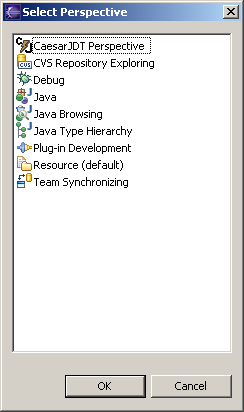
\includegraphics[width=0.3\textwidth]{images/select_persp.png}

The visualization perspective opens:\\\\
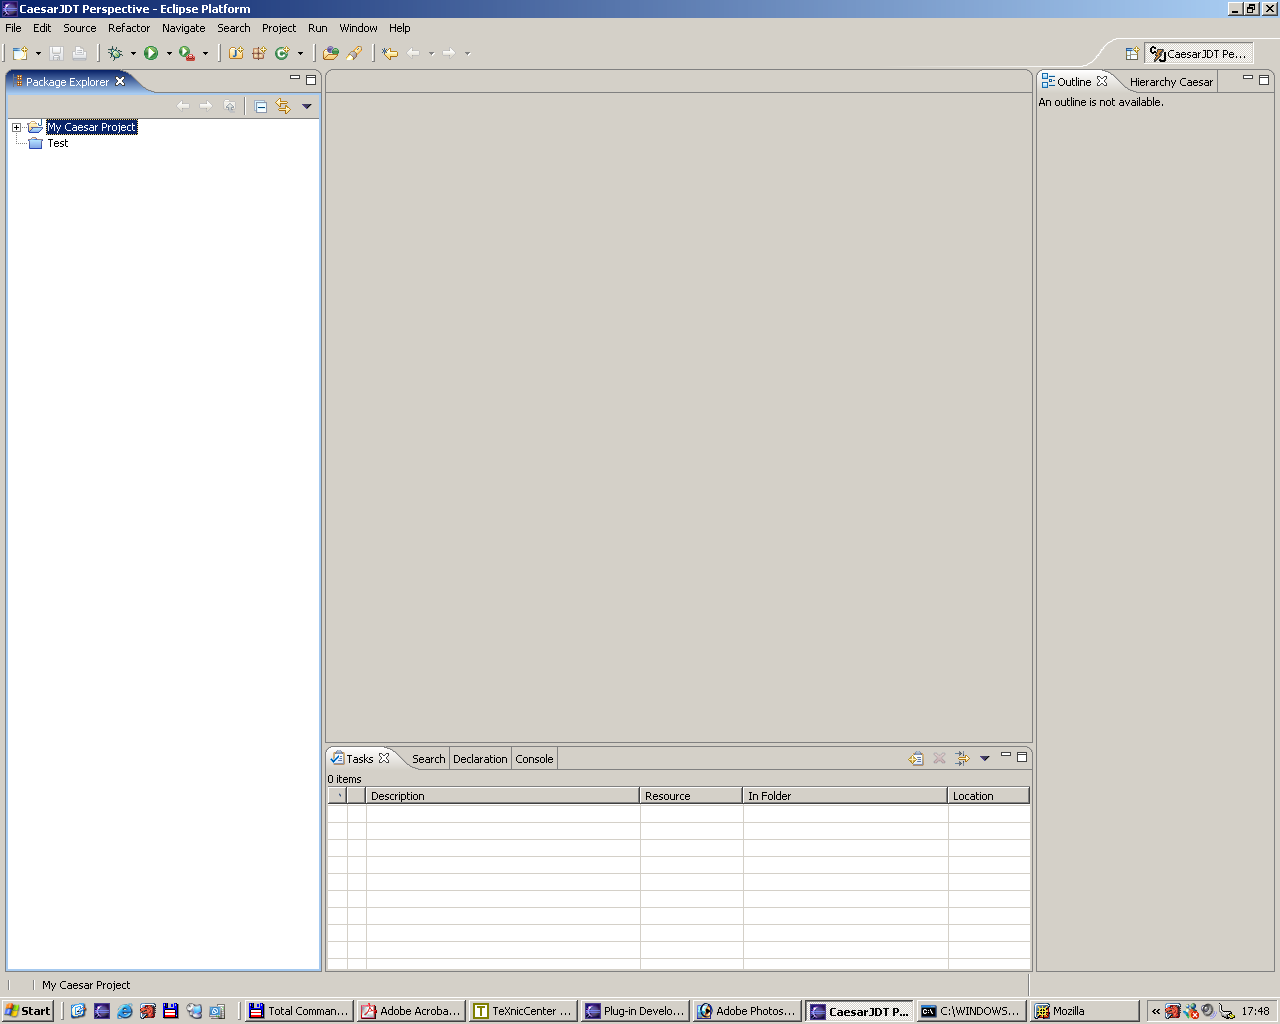
\includegraphics[width=0.7\textwidth]{images/openpersp.png}\\\\

You can switch between the Java and Caesar Visualization perspectives using the perspective icons in the top right of the menu bar.\newpage

Outline view showing structural members and crosscutting relationships (e.g. from an advice declaration to the places it advises):\\\\
\textbf{TODO BILD GEHT NICHT RICHTIG ASPECTE FEHLEN}\\
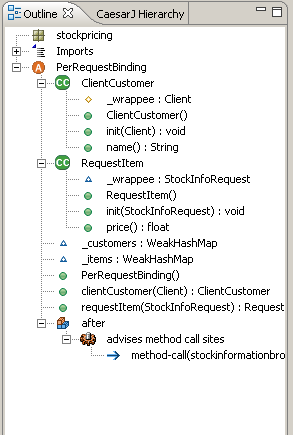
\includegraphics[width=0.30\textwidth]{images/outline.png}\\\\

A Caesar Hierarchy view showing the Typhierachy and the Linearhierarchy of an Caesar-CClass:\\\\
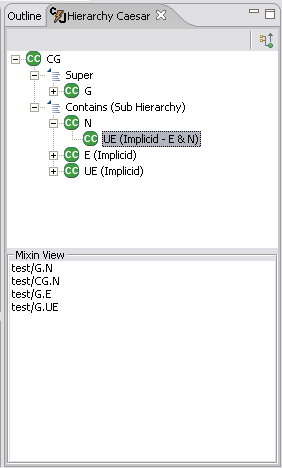
\includegraphics[width=0.30\textwidth]{images/hierarchy.png}
